The Channel System(CS) that represents the C2 System ($CS_{C2}$) is an abstraction composed by the PGs shown in Section~\ref{pg} and all exchange data structure called channels. From this model is possible to instantiate members with one or more roles and define their interactions. As our CS is parameterized, i.e., the program graphs instantiating is done according to the parameters passed, we have the following parameters:

\begin{itemize}
    \item T : set of tasks that defines the initial mission
    \item E : set of members $e_i$ that composes the team that is defined by the tuples $\langle FM, c_0\rangle$, where $FM$ is the feature model and $c_0$ is the initial valid configuration of the FM. 
    \item $\omega_0$ : the initial C2 approach ($C2_{ap}$) operated by the system
\end{itemize}

Based on this, we can define the CS as a parameterized function show by Equation \ref{CS01}. Its graphical representation is shown by Figure \ref{cs02}.

\begin{equation}
\label{CS01}
\begin{aligned}
CS_{C2}(&[e_1, e_2, ..., e_n]\ E,\ [t_1, t_2, ..., t_n]\ T,\ C2_{ap}\ \omega_0) = \\
&[C2A(E,T,\omega_0)\ |\ TA\ |\ EX(e_1, \omega_0)\ |\ EX(e_2, \omega_0)\ |...|\ EX(e_n, \omega_0)]
\end{aligned}
\end{equation}

where each member $e_k$ of the list E of members, i.e., the team, is represented by the pair $e_k=\langle FM_k,c_{0_k} \rangle$ composed by the feature model and the initial configuration of the member, the $t_k$ is the k\textit{th} task of the set T, and $\omega_0$ is the initial C2 Approach ($C2_{ap}$) operated by the team E. The total number of members, i.e., $n=|E|$, defines the quantity of Executor role instances. Each PG that forms the CS receives attributes as argument in order to create the correct diagram and they are used to satisfy their initial guard condition $g_0$.

As a result of the crosscutting concern that occurs with the roles in terms of execution (Section~\ref{sec:roles})~\cite{Apel2013}, we can observe that C2A and TA roles appear only once, even when instantiated. Similar to features scattering over different components, these roles are executed in parts and the result is the sum of each member execution. On the other hand, the EX role execution is totally performed for each member that plays this role. 

The formula \ref{CS01} represents the CS with $n$ instances of executors in a general view, that is represented by the following diagram.

\begin{figure}[h]
\centering
\label{cs02}
\scalebox{1}{


\tikzset{every picture/.style={line width=0.75pt}} %set default line width to 0.75pt        

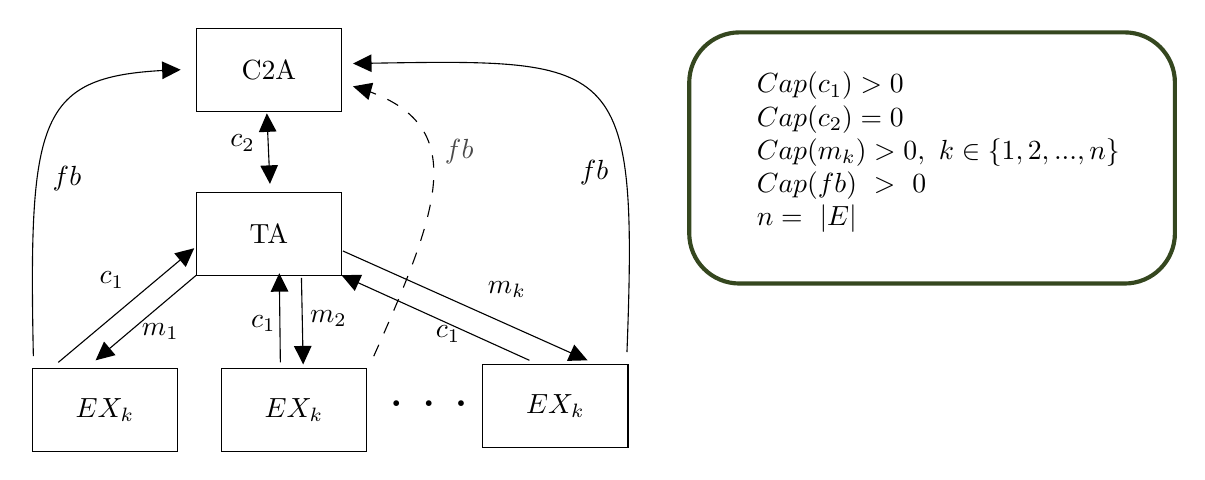
\begin{tikzpicture}[x=0.75pt,y=0.75pt,yscale=-1,xscale=1]
%uncomment if require: \path (0,229); %set diagram left start at 0, and has height of 229

%Shape: Rectangle [id:dp7793135649662085] 
\draw   (105,88) -- (175,88) -- (175,128) -- (105,128) -- cycle ;
%Shape: Rectangle [id:dp8388066725390221] 
\draw   (105,9) -- (175,9) -- (175,49) -- (105,49) -- cycle ;
%Shape: Rectangle [id:dp48691256180587716] 
\draw   (26,173) -- (96,173) -- (96,213) -- (26,213) -- cycle ;
%Straight Lines [id:da3337977868298102] 
\draw    (139.13,53) -- (140.37,81) ;
\draw [shift={(140.5,84)}, rotate = 267.47] [fill={rgb, 255:red, 0; green, 0; blue, 0 }  ][line width=0.08]  [draw opacity=0] (8.93,-4.29) -- (0,0) -- (8.93,4.29) -- cycle    ;
\draw [shift={(139,50)}, rotate = 87.47] [fill={rgb, 255:red, 0; green, 0; blue, 0 }  ][line width=0.08]  [draw opacity=0] (8.93,-4.29) -- (0,0) -- (8.93,4.29) -- cycle    ;
%Straight Lines [id:da7136052167478543] 
\draw    (155.67,129.33) -- (156.44,168) ;
\draw [shift={(156.5,171)}, rotate = 268.85] [fill={rgb, 255:red, 0; green, 0; blue, 0 }  ][line width=0.08]  [draw opacity=0] (8.93,-4.29) -- (0,0) -- (8.93,4.29) -- cycle    ;
%Straight Lines [id:da1199439366931846] 
\draw    (38.5,170) -- (101.7,116.93) ;
\draw [shift={(104,115)}, rotate = 499.98] [fill={rgb, 255:red, 0; green, 0; blue, 0 }  ][line width=0.08]  [draw opacity=0] (8.93,-4.29) -- (0,0) -- (8.93,4.29) -- cycle    ;
%Rounded Rect [id:dp3574279176331121] 
\draw  [color={rgb, 255:red, 53; green, 71; blue, 31 }  ,draw opacity=1 ][line width=1.5]  (342.5,35.2) .. controls (342.5,21.83) and (353.33,11) .. (366.7,11) -- (552.3,11) .. controls (565.67,11) and (576.5,21.83) .. (576.5,35.2) -- (576.5,107.8) .. controls (576.5,121.17) and (565.67,132) .. (552.3,132) -- (366.7,132) .. controls (353.33,132) and (342.5,121.17) .. (342.5,107.8) -- cycle ;
%Curve Lines [id:da7275055445236782] 
\draw    (26.5,167) .. controls (24.03,48.2) and (29.39,31.33) .. (95.48,29.06) ;
\draw [shift={(97.5,29)}, rotate = 538.3199999999999] [fill={rgb, 255:red, 0; green, 0; blue, 0 }  ][line width=0.08]  [draw opacity=0] (8.93,-4.29) -- (0,0) -- (8.93,4.29) -- cycle    ;
%Shape: Rectangle [id:dp8070909053866772] 
\draw   (243,171) -- (313,171) -- (313,211) -- (243,211) -- cycle ;
%Shape: Rectangle [id:dp18131918632628874] 
\draw   (117,173) -- (187,173) -- (187,213) -- (117,213) -- cycle ;
%Straight Lines [id:da4580469739796602] 
\draw    (145.5,170) -- (145.03,130) ;
\draw [shift={(145,127)}, rotate = 449.33] [fill={rgb, 255:red, 0; green, 0; blue, 0 }  ][line width=0.08]  [draw opacity=0] (8.93,-4.29) -- (0,0) -- (8.93,4.29) -- cycle    ;
%Straight Lines [id:da23459308482895536] 
\draw    (265.5,169) -- (177.73,129.24) ;
\draw [shift={(175,128)}, rotate = 384.37] [fill={rgb, 255:red, 0; green, 0; blue, 0 }  ][line width=0.08]  [draw opacity=0] (8.93,-4.29) -- (0,0) -- (8.93,4.29) -- cycle    ;
%Straight Lines [id:da9340034396500284] 
\draw    (175.67,116.33) -- (290.76,167.78) ;
\draw [shift={(293.5,169)}, rotate = 204.07999999999998] [fill={rgb, 255:red, 0; green, 0; blue, 0 }  ][line width=0.08]  [draw opacity=0] (8.93,-4.29) -- (0,0) -- (8.93,4.29) -- cycle    ;
%Straight Lines [id:da26523318096149495] 
\draw    (105,128) -- (58.79,167.06) ;
\draw [shift={(56.5,169)}, rotate = 319.78999999999996] [fill={rgb, 255:red, 0; green, 0; blue, 0 }  ][line width=0.08]  [draw opacity=0] (8.93,-4.29) -- (0,0) -- (8.93,4.29) -- cycle    ;
%Curve Lines [id:da641554832923748] 
\draw    (312.5,165) .. controls (317.97,20.72) and (308.59,23.96) .. (182.41,25.97) ;
\draw [shift={(180.5,26)}, rotate = 359.1] [fill={rgb, 255:red, 0; green, 0; blue, 0 }  ][line width=0.08]  [draw opacity=0] (8.93,-4.29) -- (0,0) -- (8.93,4.29) -- cycle    ;
%Curve Lines [id:da09438027167232854] 
\draw  [dash pattern={on 4.5pt off 4.5pt}]  (190.5,167) .. controls (223.5,93.12) and (237.09,54.18) .. (183.02,37.74) ;
\draw [shift={(180.5,37)}, rotate = 375.68] [fill={rgb, 255:red, 0; green, 0; blue, 0 }  ][line width=0.08]  [draw opacity=0] (8.93,-4.29) -- (0,0) -- (8.93,4.29) -- cycle    ;

% Text Node
\draw (140,29) node   [align=left] {C2A};
% Text Node
\draw (140,108) node   [align=left] {TA};
% Text Node
\draw (61,193) node    {$EX_{k}$};
% Text Node
\draw (64.33,130.33) node    {$c_{1}$};
% Text Node
\draw (168.67,149) node    {$m_{2}$};
% Text Node
\draw (127.33,64.33) node    {$c_{2}$};
% Text Node
\draw (462.5,69) node    {$ \begin{array}{l}
Cap( c_{1})  >0\\
Cap( c_{2}) =0\\
Cap( m_{k})  >0,\ k\in \{1,2,...,n\}\\
Cap( fb) \  >\ 0\\
n=\ |E|\ 
\end{array}$};
% Text Node
\draw (42.67,81.67) node    {$fb$};
% Text Node
\draw (278,191) node    {$EX_{k}$};
% Text Node
\draw (152,193) node    {$EX_{k}$};
% Text Node
\draw (217,190) node  [font=\Large] [align=left] {\textbf{. . .}};
% Text Node
\draw (254.67,135) node    {$m_{k}$};
% Text Node
\draw (87.67,155) node    {$m_{1}$};
% Text Node
\draw (137.33,151.33) node    {$c_{1}$};
% Text Node
\draw (226.33,156.33) node    {$c_{1}$};
% Text Node
\draw (296.67,78.67) node    {$fb$};
% Text Node
\draw (231.67,68.67) node  [color={rgb, 255:red, 74; green, 74; blue, 74 }  ,opacity=1 ]  {$fb$};


\end{tikzpicture}}
\caption{Channel System with PG instances}
\end{figure}
